\section{放出試験(大野・奥山)}
\label{chap:ejectiontest}

\subsection{計測の目的}

第\ref{chap:shapemeasurement}章で述べたように,衛星のレールは$\pm$Zを除く側面について,E-SSODのガイドレールと少なくとも75\%以上接触面を持つことがICDにより定められている.3Uである本衛星の場合は255.4mm以上のレールが必要ということになる.しかし,本衛星のレールには以下の図\ref{fig:hole}のような固定用ネジのための座繰りが設けられている.

\begin{figure}[h]
	\begin{center}
		
		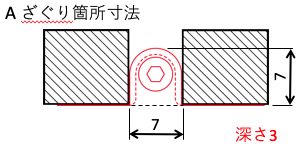
\includegraphics[width=0.6\linewidth]{04/fig/hole.png}
		\caption{ネジ穴の座繰り}
		\label{fig:hole}
		
	\end{center}
\end{figure}

この座繰りがなければレールの長さは256.5mmと要求を満たすが,座繰りによってレール長さは228.5mmとなり要求を満たさない.そのため,E-SSODから引っかかりなく本衛星がすべり出ることを確認するために,放出試験の実施がJAXA,IAより求められた.具体的な試験項目として,以下の2つが要求された.

\begin{enumerate}
	\item ポッドから衛星を水平に引出し,引出す際の力を測定することで,動摩擦係数を求める
	\item ポッドから衛星を垂直に1m/sの速さで引き抜く
\end{enumerate}

水平引き出し試験は定量的に衛星がすべり出ることができるか評価し,垂直引き出し試験では定性的に衛星が引っかかりなくすべり出ることができるかを評価する.各試験の詳細は,放出試験水平引き出し試験報告書,放出試験垂直引き抜き試験報告書(OP-S1-0099)を参照のこと.

\subsection{水平引き出し試験}

\subsubsection{試験機器}

引き出し試験は,引出すためのケブラーケーブルを放出検知ピンの穴から通したEMで行った.このEMは重量をFMと揃えるために鉛製の重りをSAP土台に取り付け調整を行なっている.ポッドはE-SSODと同じサイズである振動試験用PODを用いた.ポッドから引き出す先として,厚さ2mmのテフロンシートを敷いた台を作成した.これは衛星とPODとの動摩擦係数を測定するために,引き出した後のレール部分の摩擦を少なくするためである.以上の試験機器による実験系を以下の図\ref{fig:horizontalequipment}に示す.

\begin{figure}[h]
	\begin{center}
		
		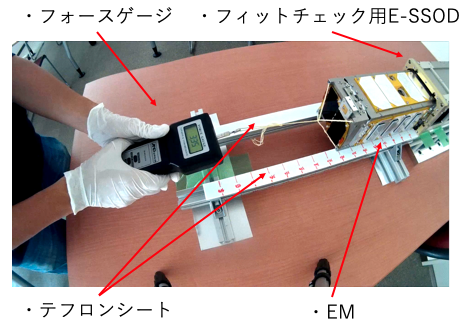
\includegraphics[width=0.6\linewidth]{04/fig/horizontalequipment.png}
		\caption{水平引き出し試験機器}
		\label{fig:horizontalequipment}
		
	\end{center}
\end{figure}

\subsubsection{試験方法}

\begin{enumerate}
	\item ポッドからテフロンシート上に衛星を引き出し,引き出し力をフォースゲージで測定し,動画で撮影する
	\item X$\pm$,Y $\pm$の各面をそれぞれ上面にした4通りで測定を行う
	\item 試験結果動画から30mmごとに引き出し力を記録し,動摩擦力を計算する
\end{enumerate}

\subsubsection{評価方法}

IHIから動摩擦係数が0.1程度であることが要求されたため,測定値と要求値を比較することで評価する.

\subsubsection{試験結果}

まず,1階の実験室クリーンブース内(温度23.5$^\circ$C,湿度81$\%$)で行なった.その結果,放出の前半における動摩擦係数が0.15$\sim$0.17,放出後半で0.12$\sim$0.15程度であった.この結果は,要求値とオーダーがずれておらず問題ないと考えIAに結果を提出したが,動摩擦係数の値が大きいとの返答であった.また,IAから多湿な環境で実験を行うと動摩擦係数が大きくなるため,低湿度下での実験を求められた.

そこで,5階の実験室(温度25$^\circ$C,湿度65$\%$)で再実験を行なった.その結果,放出の前半における動摩擦係数が0.10$\sim$0.15,放出後半で0.09$\sim$0.13程度となり,JAXA,IAから承認を得た.

\subsection{垂直引き出し試験}

\subsubsection{試験機器}

水平引き出し試験と同様に,引き出し用ケブラー糸を取り付け,鉛重りで重量を調整したEMと振動試験用ポッドを用いて実験を行なった.振動試験用ポッドには誤って衛星が落下した際の衝撃防止としてスタイロフォームを貼り付けた.また,垂直に1m/sで引き出すために定滑車を用いた.実験系は以下の図のようになった.

\begin{figure}[h]
	\begin{center}
		
		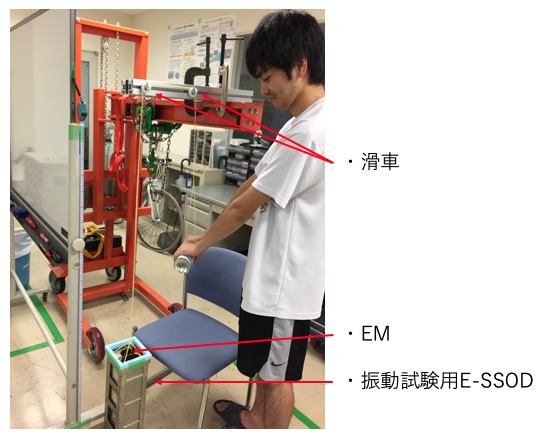
\includegraphics[width=0.6\linewidth]{04/fig/verticalequipment.png}
		\caption{垂直引き出し試験機器}
		\label{fig:verticalequipment}
		
	\end{center}
\end{figure}

\subsubsection{試験方法}

\begin{enumerate}
\item 定滑車を介した紐を引っ張りポッドから衛星を引き抜く様子を動画で撮影する
\item 試験結果動画から引き抜き時に引っかかりがないかを確認する
\item 試験結果動画から引き抜き速さを計算する
\end{enumerate}

\subsubsection{評価方法}

衛星が引っかかりなく引き出せているか,引き抜き速さが1m/s程度になっているかによって評価する.

\subsubsection{試験結果}

衛星は引っかかりなく引き出すことができた.また,衛星長さ340.5mmの引き出しに0.3sかかっていたため,引き抜き速さはおよそ1.1m/sであった.以上の結果からJAXA,IAから承認を得ることができた.